\documentclass[a4paper,12pt]{article}
\usepackage[T2A]{fontenc}
\usepackage[utf8]{inputenc}
\usepackage[russian]{babel}
\usepackage{graphicx}
\usepackage{amsmath, amssymb}
\usepackage{geometry}
\usepackage{listings}
\usepackage{tikz}
\usepackage[hidelinks]{hyperref}

\usetikzlibrary{positioning}

\geometry{left=2cm, right=2cm, top=2cm, bottom=2cm}


\title{Учебный проект: БД зоомагазина "Лап-Ландия" и её интересное окружение}

\author{Александр Гоппе}
\date{}


\begin{document}

    \maketitle

    \begin{center}
        
\includegraphics[width=0.7\textwidth]{title} % Вставка изображения
    \end{center}

    \vfill
    \begin{center}
        \date{\today}
    \end{center}
    \newpage

    \tableofcontents
    \newpage

    \section{Описание проекта}\label{sec:-projectdesc-}
    Учебный проект \textbf{Лап-Ландия} посвящён построению базы данных для зоомагазина с развёрнутой инфраструктурой,
включающей реплицируемую БД, балансировщик нагрузки,
инструменты мониторинга и анализатора данных, а также
серверного и клиентского приложений, работающих с данными.
Демонстрационный стенд разворачивается ``по клику`` через docker compose.

\subsection{Общая структура}\label{subsec:generalstructure}

\begin{itemize}
    \item \textbf{База данных}: кластер Patroni из трёх узлов.
    \item \textbf{Балансировка}: HAProxy (1 демонстрационный экземпляр).
    \item \textbf{Распределённая Система Контроля (DCS)}: Zookeeper 3 экземпляра.
    \item \textbf{Инициализация БД}: мини-контейнер db-script-runner (создаёт базу и юзеров).
    \item \textbf{Миграции}: Flyway.
    \item \textbf{Мониторинг}: PostgreSQL Exporter + Prometheus + Grafana.
    \item \textbf{Бизнес-аналитика}: Apache Superset.
    \item \textbf{Демонстрационное приложение}: Spring Boot (Java) + JPA (Hibernate).
    \item \textbf{Демонстрационное тестирование API}: контейнер curl\_runner (отправляет запросы в приложение).
    \item \textbf{Фронт}: React.js.
    \item \textbf{Логирование в ClickHouse}: через Logstash.
\end{itemize}

Один экземпляр балансировщика HAProxy был развёрнут с пониманием того, что в реальном производстве их должно быть
минимум два.
Но, т.к. всё окружение разворачивается в тестовой среде на персональном компьютере ученика и точка отказа, так или
иначе, одна - работает один экземпляр.
Теоретически можно было бы обойтись двумя узлами Zookeeper и Patroni, но, как и многое в этом проекте, эти настройки
были взяты из открытых источников и, ввиду и без того не самой тривиальной архитектуры стенда, было решено
не тратить время на переделку готовых наработок коллег-ремесленников.

Аналогично не реплицировались Superset, ClickHouse и другие системы, т.к. предпочтительной задачей в контексте курса
была выбрана настройка некоторого одного ``целевого`` кластера СУБД.

\newpage

\subsection{Диаграмма инфраструктуры}\label{subsec:structurediagram}

\begin{figure}[h]
    \centering
    \resizebox{\textwidth}{!}{%
        \begin{tikzpicture}

            \node (app) [draw, rectangle, rounded corners, minimum width=3cm, minimum height=1cm] {Java-приложение};
            \node (haproxy) [draw, rectangle, rounded corners, minimum width=3cm, minimum height=1cm, below=of app] {HAProxy};
            \node (db1) [draw, rectangle, rounded corners, minimum width=3cm, minimum height=1cm, below left=of haproxy] {Patroni 1};
            \node (db2) [draw, rectangle, rounded corners, minimum width=3cm, minimum height=1cm, below=of haproxy] {Patroni 2};
            \node (db3) [draw, rectangle, rounded corners, minimum width=3cm, minimum height=1cm, below right=of haproxy] {Patroni 3};
            \node (zookeeper) [draw, rectangle, below=of db2, minimum width=3cm, minimum height=1cm] {Zookeeper (3 экз.)};
            \node (flyway) [draw, rectangle, rounded corners, minimum width=3cm, minimum height=1cm, below=of db1] {Flyway, db-init};
            \node (superset) [draw, rectangle, rounded corners, minimum width=3cm, minimum height=1cm, right=of haproxy] {Superset};
            \node (logstash) [draw, rectangle, rounded corners, minimum width=3cm, minimum height=1cm, above=of app] {LogStash};
            \node (front) [draw, rectangle, rounded corners, minimum width=3cm, minimum height=1cm, right=of app] {Front/Curl};
            \node (clickhouse) [draw, rectangle, rounded corners, minimum width=3cm, minimum height=1cm, above right=of app] {ClickHouse};
            \node (pgexporter) [draw, rectangle, rounded corners, minimum width=3cm, minimum height=1cm, left=of haproxy] {PG-exporter};
            \node (prometheus) [draw, rectangle, rounded corners, minimum width=3cm, minimum height=1cm, above=of pgexporter] {Prometheus};
            \node (grafana) [draw, rectangle, rounded corners, minimum width=3cm, minimum height=1cm, above=of prometheus] {Grafana};

            \draw[->] (app) -- (haproxy);
            \draw[->] (superset) -- (haproxy);
            \draw[->] (haproxy) -- (db1);
            \draw[->] (haproxy) -- (db2);
            \draw[->] (haproxy) -- (db3);
            \draw[->] (zookeeper) -- (db1);
            \draw[->] (zookeeper) -- (db2);
            \draw[->] (zookeeper) -- (db3);
            \draw[->, dash pattern=on 2pt off 2pt] (flyway) -- (haproxy)
            \draw[->] (logstash) -- (clickhouse);
            \draw[->] (app) -- (logstash);
            \draw[->] (front) -- (app);
            \draw[->] (pgexporter) -- (haproxy);
            \draw[->] (prometheus) -- (pgexporter);
            \draw[->] (grafana) -- (prometheus);
        \end{tikzpicture}
    }
    \caption{Схема инфраструктуры проекта}\label{fig:structurefigure}
\end{figure}

    \section{Структура и элементы хранилища данных}\label{sec:-dbstructure-}
    \subsection{Схемы}\label{subsec:schemas}
В базе созданы следующие схемы:
\begin{itemize}
    \item \textbf{archive}: архивированные данные, для разгрузки оперативной схемы.
    \item \textbf{business}: оперативная схема с данными о покупках в сети зоомагазинов.
    \item \textbf{cron}: техническая схема для элементов расширения cron.
    \item \textbf{migrations}: техническая схема инструмента миграции flyway.
    \item \textbf{public}: общая начальная схема PostgreSQL\@.
\end{itemize}

\subsection{Схема archive: описание}\label{subsec:archive}

Архивируются только данные о покупках, как наиболее тяжёлые и интенсивные.
Структура и индексы полностью дублируют прототипы из бизнес-схемы.

\subsection{Схема business: описание}\label{subsec:business}

Оперативные бизнес-данные о покупках, магазинах, покупателях.

\begin{figure}[h]
    \centering
    \resizebox{\textwidth}{!}{%
        \begin{tikzpicture}[
            node distance=2cm and 3cm,
            every node/.style={draw, rectangle, rounded corners, minimum width=3cm, minimum height=1cm, align=center}
        ]
            % Определяем таблицы
            \node (category) {category};
            \node (product) [below=of category] {product};
            \node (inventory) [left=of product] {inventory};
            \node (shop) [below=of inventory] {shop};
            \node (supplier) [right=of product] {supplier};
            \node (purchase) [below=of product] {purchase};
            \node (purchase_item) [right=of purchase] {purchase\_item};
            \node (customer) [below=of purchase] {customer};

            % Связи между таблицами
            \draw[->] (product) -- (category);
            \draw[->] (product) -- (supplier);
            \draw[->] (inventory) -- (shop);
            \draw[->] (inventory) -- (product);
            \draw[->] (purchase) -- (customer);
            \draw[->] (purchase) -- (shop);
            \draw[->] (purchase_item) -- (purchase);
            \draw[->] (purchase_item) -- (product);
        \end{tikzpicture}
    }
    \caption{Схема связей таблиц}\label{fig:figure-tables}
\end{figure}

\subsubsection{Таблица category}

\begin
    \normalsize
    \renewcommand{\arraystretch}{1.5} % Регулируем высоту строк
    \begin{tabular}{|l|l|l|}
        \hline
        \textbf{Имя столбца} & \textbf{Тип} & \textbf{Описание}                  \\
        \hline
        id                   & SERIAL       & Уникальный идентификатор категории \\
        \hline
        name                 & TEXT         & Название категории                 \\
        \hline
    \end{tabular}
\end

\subsubsection{Таблица product}

\begin
    \normalsize
    \renewcommand{\arraystretch}{1.5} % Регулируем высоту строк
    \begin{tabular}{|l|l|l|}
        \hline
        \textbf{Имя столбца} & \textbf{Тип}  & \textbf{Описание}                      \\
        \hline
        id                   & SERIAL        & Уникальный идентификатор продукта      \\
        \hline
        name                 & TEXT          & Название продукта                      \\
        \hline
        description          & TEXT          & Описание продукта                      \\
        \hline
        category\_id         & INT           & Ссылка на категорию (category.id)      \\
        \hline
        price                & NUMERIC(10,2) & Цена продукта                          \\
        \hline
        characteristics      & JSONB         & Характеристики продукта в формате JSON \\
        \hline
    \end{tabular}
\end

\subsubsection{Таблица shop}

\begin
    \normalsize
    \renewcommand{\arraystretch}{1.5} % Регулируем высоту строк
    \begin{tabular}{|l|l|l|}
        \hline
        \textbf{Имя столбца} & \textbf{Тип} & \textbf{Описание}                 \\
        \hline
        id                   & SERIAL       & Уникальный идентификатор магазина \\
        \hline
        name                 & TEXT         & Название магазина                 \\
        \hline
        location             & TEXT         & Местоположение магазина           \\
        \hline
    \end{tabular}
\end

\subsubsection{Таблица inventory}

\begin
    \normalsize
    \renewcommand{\arraystretch}{1.5} % Регулируем высоту строк
    \begin{tabular}{|l|l|l|}
        \hline
        \textbf{Имя столбца} & \textbf{Тип} & \textbf{Описание}              \\
        \hline
        shop\_id             & INT          & Ссылка на магазин (shop.id)    \\
        \hline
        product\_id          & INT          & Ссылка на продукт (product.id) \\
        \hline
        quantity             & INT          & Количество товара в магазине   \\
        \hline
    \end{tabular}
\end

\subsubsection{Таблица supplier}

\begin
    \normalsize
    \renewcommand{\arraystretch}{1.5} % Регулируем высоту строк
    \begin{tabular}{|l|l|l|}
        \hline
        \textbf{Имя столбца} & \textbf{Тип} & \textbf{Описание}                   \\
        \hline
        id                   & SERIAL       & Уникальный идентификатор поставщика \\
        \hline
        name                 & TEXT         & Название поставщика                 \\
        \hline
        contact\_info        & TEXT         & Контактная информация поставщика    \\
        \hline
    \end{tabular}
\end

\subsubsection{Таблица customer}

\begin
    \normalsize
    \renewcommand{\arraystretch}{1.5} % Регулируем высоту строк
    \begin{tabular}{|l|l|l|}
        \hline
        \textbf{Имя столбца} & \textbf{Тип}    & \textbf{Описание}                  \\
        \hline
        id                   & SERIAL          & Уникальный идентификатор клиента   \\
        \hline
        phone                & phone\_domain   & Телефон клиента                    \\
        \hline
        email                & email\_domain   & Электронная почта клиента          \\
        \hline
        name                 & TEXT            & Имя клиента                        \\
        \hline
        loyalty\_status      & loyalty\_status & Статус лояльности клиента          \\
        \hline
        bonus\_points        & NUMERIC(10,2)   & Количество бонусных баллов клиента \\
        \hline
    \end{tabular}
    \vspace{10pt} % или \bigskip, если нужно побольше
\end

Несмотря на предполагаемую валидацию на бэкенде, правильные базовые типы в целом в базе не помешают.
Перечисление поможет избежать случайных описок и логически ограничит значения.

\subsubsection{Таблица purchase}

\begin
    \normalsize
    \renewcommand{\arraystretch}{1.5} % Регулируем высоту строк
    \begin{tabular}{|l|l|l|}
        \hline
        \textbf{Имя столбца} & \textbf{Тип}  & \textbf{Описание}                \\
        \hline
        id                   & BIGSERIAL     & Уникальный идентификатор покупки \\
        \hline
        customer\_id         & INT           & Ссылка на клиента (customer.id)  \\
        \hline
        shop\_id             & INT           & Ссылка на магазин (shop.id)      \\
        \hline
        purchase\_date       & TIMESTAMP     & Дата покупки                     \\
        \hline
        total\_amount        & NUMERIC(10,2) & Общая сумма покупки              \\
        \hline
    \end{tabular}
    \vspace{10pt} % или \bigskip, если нужно побольше
\end

Используем BIGSERIAL для подстраховки от переполнения номеров покупок.

\subsubsection{Таблица purchase\_item}

\begin
    \normalsize
    \renewcommand{\arraystretch}{1.5} % Регулируем высоту строк
    \begin{tabular}{|l|l|l|}
        \hline
        \textbf{Имя столбца} & \textbf{Тип} & \textbf{Описание}               \\
        \hline
        purchase\_id         & BIGINT       & Ссылка на покупку (purchase.id) \\
        \hline
        product\_id          & INT          & Ссылка на продукт (product.id)  \\
        \hline
        quantity             & INT          & Количество товара в покупке     \\
        \hline
    \end{tabular}
\end

\subsubsection{Индексы}

\begin{center}
    \resizebox{\textwidth}{!}{%
        \begin{tabular}{|l|l|l|}
            \hline
            \textbf{Имя индекса}          & \textbf{Таблица} & \textbf{Описание}                                                           \\
            \hline
            idx\_product\_search          & product          & Индекс для поиска по описанию и характеристикам продукта (используется GIN) \\
            \hline
            idx\_product\_category        & product          & Индекс по категории продукта (category\_id)                                 \\
            \hline
            idx\_inventory\_product\_shop & inventory        & Индекс по продуктам и магазинам в инвентаре                                 \\
            \hline
            idx\_purchase\_customer\_date & purchase         & Индекс по покупателю и дате покупки                                         \\
            \hline
            idx\_purchase\_brin           & purchase         & Индекс с использованием BRIN для диапазона дат покупок                      \\
            \hline
            idx\_customer\_phone          & customer         & Уникальный индекс по телефону клиента                                       \\
            \hline
        \end{tabular}
    }
\end{center}

\subsection{Пользовательские типы данных}\label{subsec:usertypes}

В данной секции приведены пользовательские типы и домены, используемые в базе данных.

\begin{itemize}
    \item \textbf{email\_domain} – текстовый тип, содержащий email-адрес.
    Соответствует регулярному выражению:
    \begin{verbatim}
^[A-Za-z0-9._%+-]+@[A-Za-z0-9.-]+\.[A-Za-z]{2,}$
    \end{verbatim}

    \item \textbf{phone\_domain} – текстовый тип для хранения телефонных номеров.
    Допустимые значения:
    \begin{verbatim}
^\+?\d{10,15}$
    \end{verbatim}

    \item \textbf{loyalty\_status} – перечислимый тип, определяющий уровень лояльности клиента.
    Возможные значения:
    \begin{center}
        \begin{tabular}{|c|c|}
            \hline
            Значение & Описание        \\
            \hline
            BRONZE   & Базовый уровень \\
            SILVER   & Средний уровень \\
            GOLD     & Высший уровень  \\
            \hline
        \end{tabular}
    \end{center}
\end{itemize}

\subsection{Процедуры, функции и задания по расписанию}\label{subsec:procedures}

В данной секции приведены хранимые процедуры, функции и задания, выполняемые в базе данных.

\subsubsection{Процедуры}

\begin{itemize}
    \item \textbf{archive\_old\_purchases} – процедура для архивации устаревших данных о покупках.
    \begin{itemize}
        \item Выполняет перенос устаревших записей в архивную таблицу.
        \item Освобождает основную таблицу от старых данных.
    \end{itemize}
\end{itemize}

\subsubsection{Функции}

\begin{itemize}
    \item \textbf{transliterate} – функция для транслитерации текста.
    \begin{itemize}
        \item Принимает строку на входе.
        \item Возвращает строку, в которой символы заменены на их латинские аналоги.
    \end{itemize}
\end{itemize}

Функция может пригодиться при миграциях и расширении БД.
В данном проекте она нашла применение для эстетичности генерируемых данных :)

\subsubsection{Задание по расписанию}

В базе используется планировщик задач для автоматического выполнения архивации старых покупок.

\begin{itemize}
    \item \textbf{Задание архивации:} выполняется ежедневно в 04:00.
\end{itemize}

\begin{lstlisting}[language=SQL, frame=single, basicstyle=\normalsize\ttfamily, breaklines=true,label={lst:cronsql}]
SELECT cron.schedule('0 4 * * *',
    $$CALL business.archive_old_purchases();$$);
\end{lstlisting}

\subsection{Схема cron: описание}\label{subsec:crondesc}

Данная схема создана подключенным в ходе инициализации БД расширением pg\_cron и содержит технические таблицы
`job` и `job\_run\_details` с информацией о заданиях.

\subsection{Схема migrations: описание}\label{subsec:migrationsdesc}

Данная схема создана используемым для управления миграциями инструментом flyway и содержит
единственную техническую таблицу `flyway\_schema\_history` с информацией о миграциях.

    \section{Обоснование модели с точки зрения нормализации}\label{sec:-normalization-}
    Проектируемая база данных зоомагазина соответствует принципам нормализации,
что позволяет минимизировать избыточность данных, устранить аномалии обновления и обеспечить целостность информации.
Рассмотрим, как наша модель удовлетворяет требованиям нормальных форм.

\subsection{Первая нормальная форма (1NF)}\label{subsec:1nf}
Первая нормальная форма требует, чтобы каждая таблица содержала только атомарные значения,
а каждая строка была уникальной.
\begin{itemize}
    \item Все атрибуты содержат неделимые значения (например, `phone` и `email` в таблице `customer`).
    \item В таблице `inventory` используется составной первичный ключ `(shop\_id, product\_id)`,
    что исключает дублирование записей о наличии товаров в магазинах.
    \item В таблице `purchase\_item` связь между покупкой и товарами организована через `purchase\_id` и `product\_id`,
    что позволяет хранить любое количество товаров в одной покупке без нарушения 1NF\@.
\end{itemize}

\subsection{Вторая нормальная форма (2NF)}\label{subsec:2nf}
Вторая нормальная форма требует выполнения 1NF и отсутствия частичных зависимостей от составного ключа.
\begin{itemize}
    \item Все таблицы, кроме `inventory` и `purchase\_item`, имеют простой первичный ключ.
    \item В `inventory` и `purchase\_item` данные зависят от обоих ключей в составном первичном ключе,
    что соответствует 2NF\@.
    \item Атрибуты зависят исключительно от идентификаторов записей, например,
    `loyalty\_status` в `customer` и `price` в `product`.
\end{itemize}

\subsection{Третья нормальная форма (3NF)}\label{subsec:3nf}
Третья нормальная форма требует, чтобы в таблице не было транзитивных зависимостей.
\begin{itemize}
    \item В таблице `customer` атрибут `loyalty\_status` является перечисляемым типом (`ENUM`),
    что предотвращает избыточность данных.
    \item Поля `category\_id` и `supplier\_id` в `product` хранят только идентификаторы,
    а полные сведения находятся в соответствующих таблицах.
    \item В `purchase` `total\_amount` хранится явно, но он не зависит от `customer\_id` или `shop\_id`,
    а вычисляется из `purchase\_item`, что не нарушает 3NF\@.
\end{itemize}

\subsection{Дополнительные аспекты нормализации}\label{subsec:normalizationadditional}
\begin{itemize}
    \item Использование **доменных типов** (`email\_domain`, `phone\_domain`)
    не только упрощает контроль данных, но и способствует нормализации, предотвращая дублирование проверок.
    \item JSONB-колонка `characteristics` в `product` допускает хранение специфических
    характеристик товаров без нарушения принципов нормализации, так как JSONB-данные не
    участвуют в ключах или зависимостях.
    \item Ограничения целостности (`CHECK`, `FOREIGN KEY`, `UNIQUE`) обеспечивают
    консистентность данных на уровне СУБД.
\end{itemize}

\subsection{Вывод}\label{subsec:normalizationresult}
Данная модель базы данных соответствует третьей нормальной форме (3NF),
обеспечивая структурированное и эффективное хранение данных.
Она балансирует между строгой нормализацией и практичностью, например,
JSONB-атрибуты добавляют гибкость без нарушения основных нормализационных требований.
Такой подход минимизирует дублирование данных, упрощает обновления и поддерживает
высокую производительность запросов.



    \section{Кластер Patroni и настройки узлов БД}\label{sec:-patronicluster-}
    \subsection{Кластер Patroni}\label{subsec:patroni}

Кластер Patroni разворачивается благодаря подготовленному образу,
включающему в себя установку различных python-библиотек и расширений и настроечный
файл patroni.yml, содержащий различные настройки для Распределённой Системы Контроля (DCS),
в качестве которой был выбран Zookeeper.
В целом, настройки любой DCS практически идентичны и подкрепляются соответствующими библиотеками python.

\begin{lstlisting}[language=YAML, frame=single, basicstyle=\normalsize\ttfamily, breaklines=true,label={lst:patroniyaml}]
bootstrap:
  dcs:
    ttl: 30
...
zookeeper:
  hosts:
    - zoo1:2181
    - zoo2:2181
    - zoo3:2181
  scope: patroni
  namespace: /service/patroni
\end{lstlisting}

\subsection{Распределённый контроль с помощью Zookeeper}\label{subsec:zookeeper}

DCS была выбрана исходя из наличия минимального знакомства с ней благодаря работе с Apache Kafka.
Zookeeper поддерживает иерархичное храрение ключей и является устоявшейся системой, и хорошо подходит для
хранения не часто меняющихся данных.
При выборе продуктового варианта, однако, можно рассмотреть выбор и ETCD, популярность которого растёт на фоне,
как принято считать, отличается более простым настраиванием и интеграцией с kubernetes.
В самом Zookeeper можно поинтересоваться данными patroni, такими как список узлов, конфигурацией, переданной для
DCS, или, например, кто сейчас является лидером:

\begin{lstlisting}[language=bash, frame=single, basicstyle=\normalsize\ttfamily, breaklines=true,label={lst:zkclish}]
$ root@zoo1:/zookeeper-3.4.14/bin# zkCli.sh
Connecting to localhost:2181
...
get /service/patroni/leader
{"leader": "patroni1", "epoch": 0}
...
\end{lstlisting}

\subsection{Балансировщик с высокой доступностью HAProxy}\label{subsec:haproxy}

HAProxy настроен на API нашего Patroni так, что healthcheck проверяет HTTP-статус 200.
Такой статус возвращает только мастер-узел, а реплики возвращают 503.

Однако, при желании или необходимости, можно разгрузить мастер-узел от чтений, добавив в HAProxy дополнительный
backend.
Это потребует от нас развить работающие с БД приложения на использование двух источников данных с балансировкой,
например, в контексте инструментария Spring Boot JPA\@.
В данной работе этот вариант только обозначим, а настроим на прямую работу только с мастером.

    \section{Мониторинг}\label{sec:-monitoring-}
    \subsection{Общее описание мониторинга}\label{subsec:monitoringall}
Мониторинг организован с помощью:

\begin{itemize}
    \item \textbf{postgres\_exporter} - инструмента, который выполняет запросы к базе, подключаясь под
    специально созданным юзером с ограниченными правами.
    \item \textbf{Prometheus} - известного сборщика метрик, обращающегося по http к postgres\_exporter.
    \item \textbf{Grafana} - инструмента визуализации метрик.
\end{itemize}

В качестве изюминки проекта было реализовано предварительное встраивание панелей (дашбордов)
при разворачивании образа grafana, делая проект готовым к демонстрации уже ``с порога``.
Готовая красивая панель для postgresql была скачана с сайта grafana.

\begin{figure}[htbp]
    \centering
    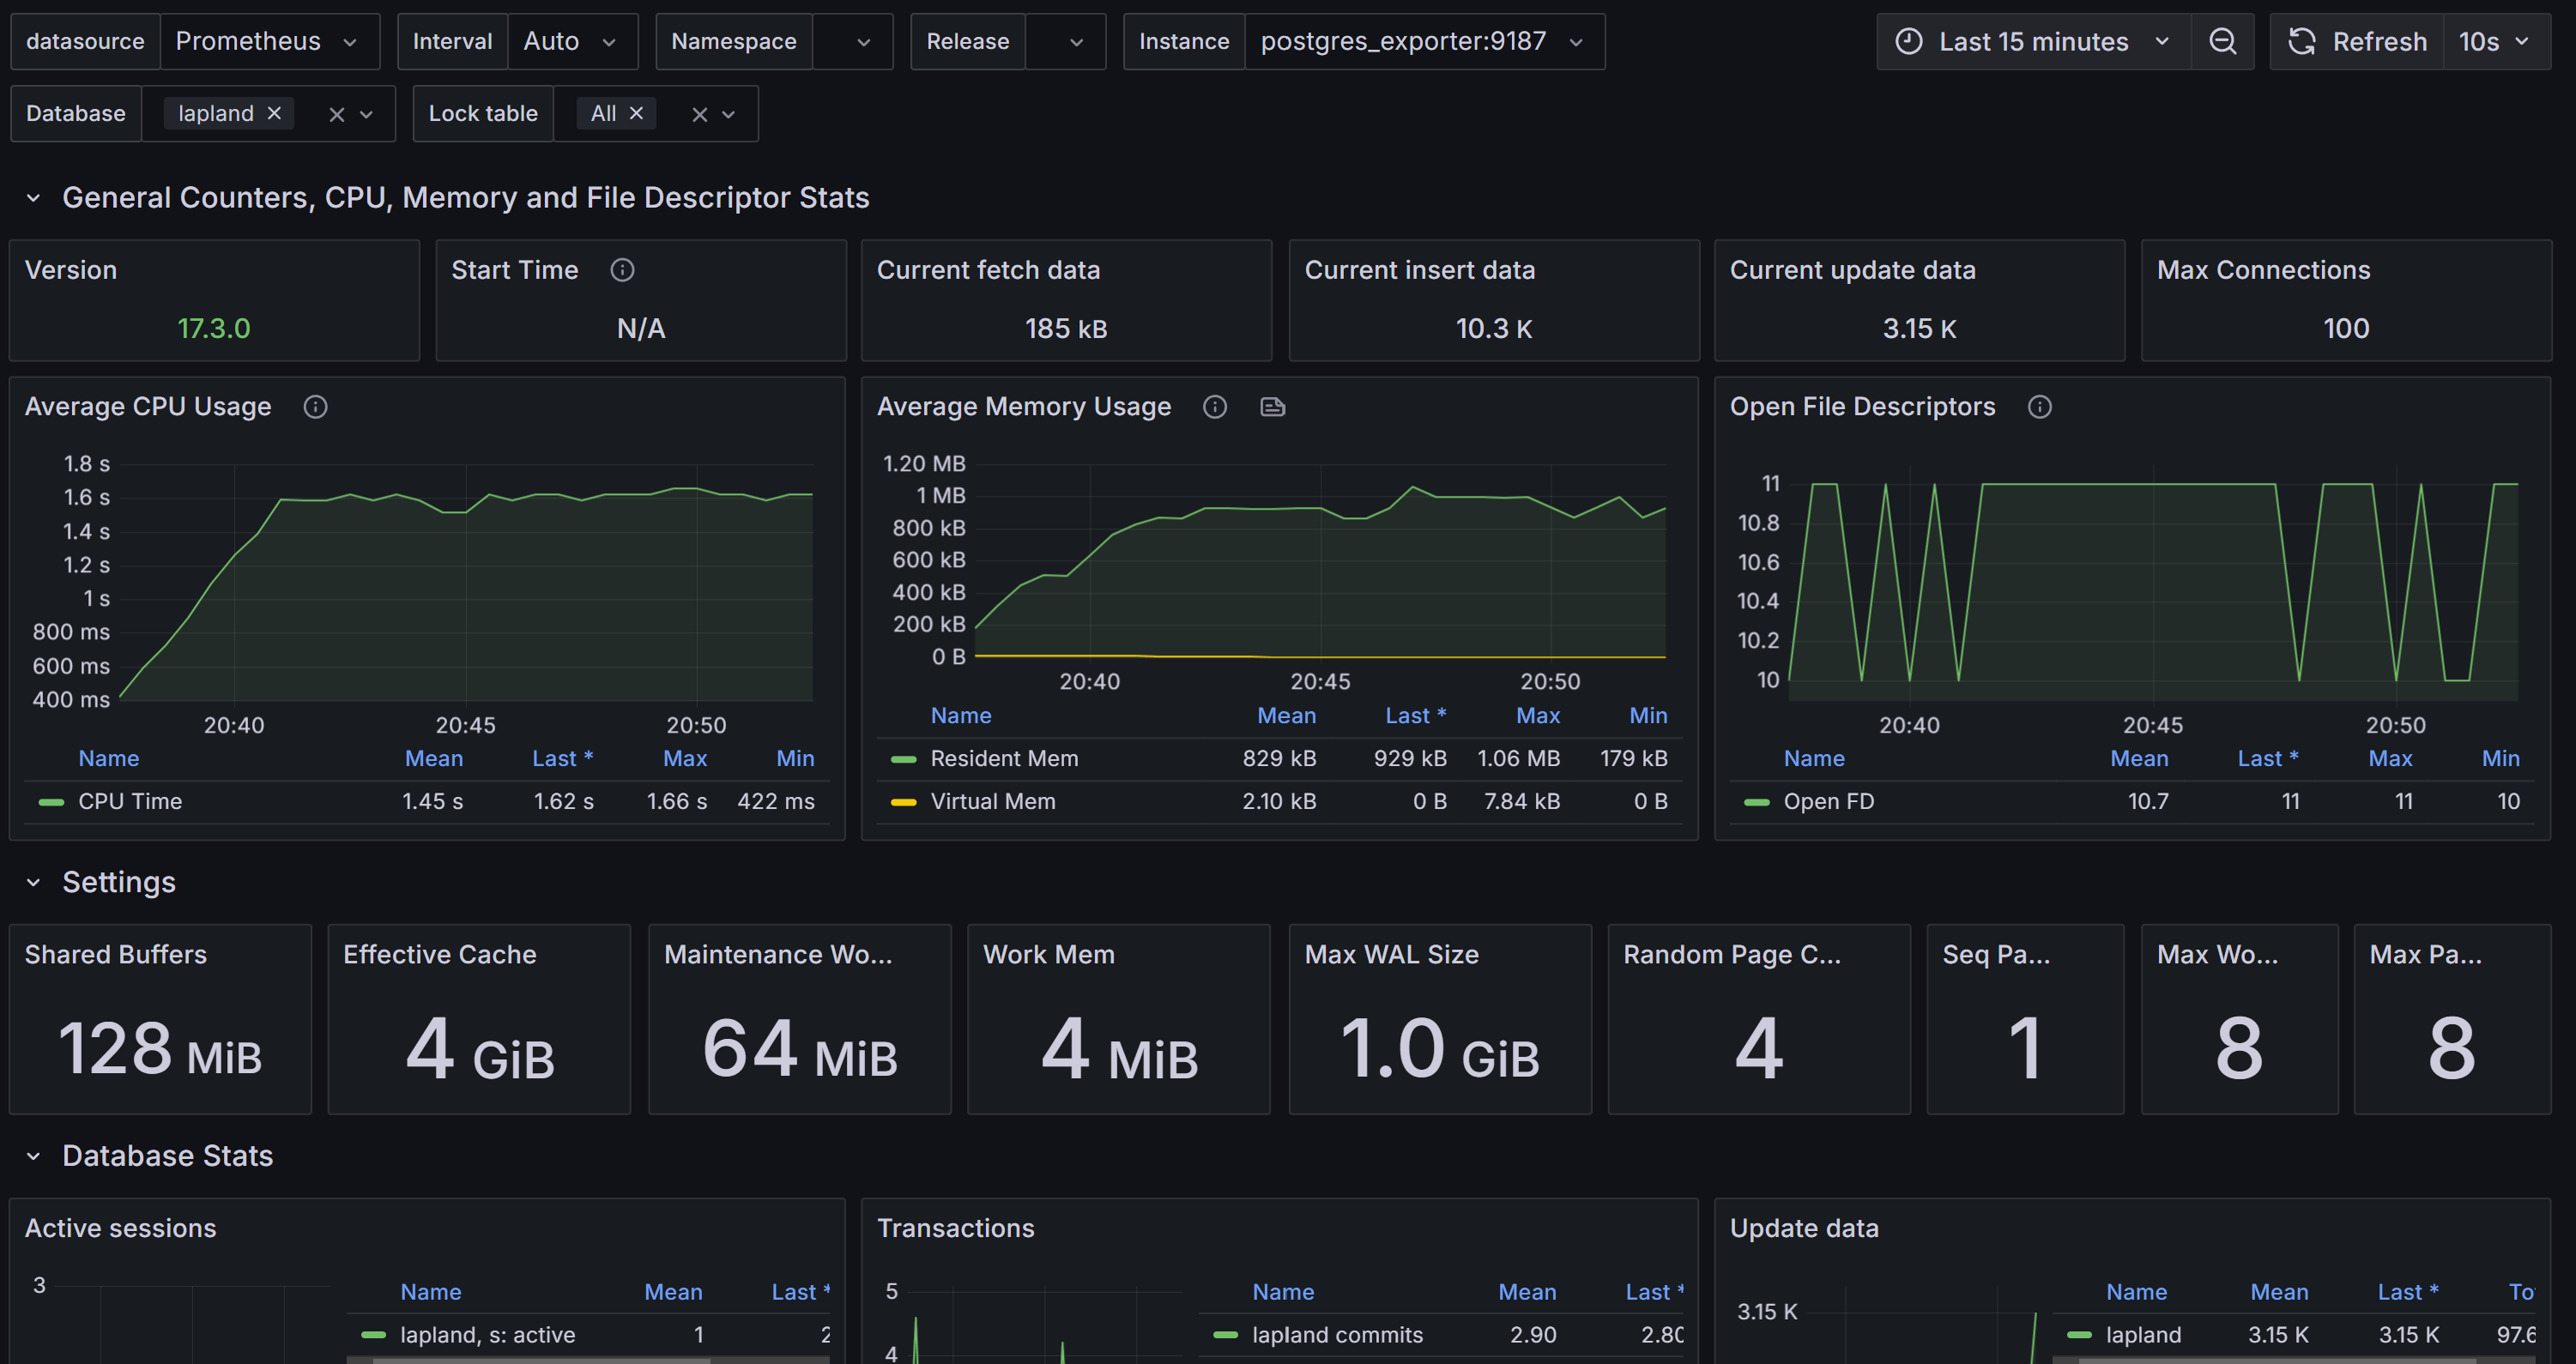
\includegraphics[width=0.9\textwidth]{grafana} % Вставка изображения
    \caption{Панель мониторинга в Grafana}\label{fig:grafanapic}
\end{figure}

    \section{Бизнес-аналитика}\label{sec:-businessintelligence-}
    \subsection{Настройка Apache Superset}\label{subsec:-apache-superset}
Это известное средство анализа и визуализации данных с открытым исходным кодом для настройки ``по кнопке``
требует ощутимого упорства.
Для автоматизации запуска Superset с предустановленными панелями потребовалась усиленная команда запуска ПО в виде:
\begin{itemize}
    \item Установки библиотек для подключения к целевой БД (PostgreSQL).
    \item Инициализации внутренней базы (которой по умолчанию является
    встроенная sqlite3, это решение хорошо подходит для демонстрации, но в продуктовой среде к использованию не
    рекомендуется).
    \item Инициализации самого Superset.
    \item Создания администратора с паролем.
    \item Ожидания запуска Superset по определённому порту.
    \item Запуска скрипта импорта с использованием API Superset, включающего:
    \begin{itemize}
        \item Получение токена для обращений по API\@.
        \item Импорту подготовленного архива с панелями и чартами.
    \end{itemize}
\end{itemize}

Существенной сложностью в отладке и построении данного процесса было диагностирование и обход требования
использования CSRF-токена для работы с flask-сервером, реализующим API Superset.
Изучались заголовки запросов в отладчике браузера, документация Superset, форумы и GPT-объяснения.
В результате в изначальные настройки программы, расположенные в python-скрипте были добавлены переменные,
отключающие механизм CSRF-токена и ослабляющие настройки безопасности на демонстрационном стенде.

\subsection{Панели}\label{subsec:supersetpanels}

Ниже приведена автоматически импортируемая панель.
График был собран из данных таблицы покупок, агрегированных по дате.
Чарт - из запроса по нескольким таблицам со связями.

\begin{figure}[htbp]
    \centering
    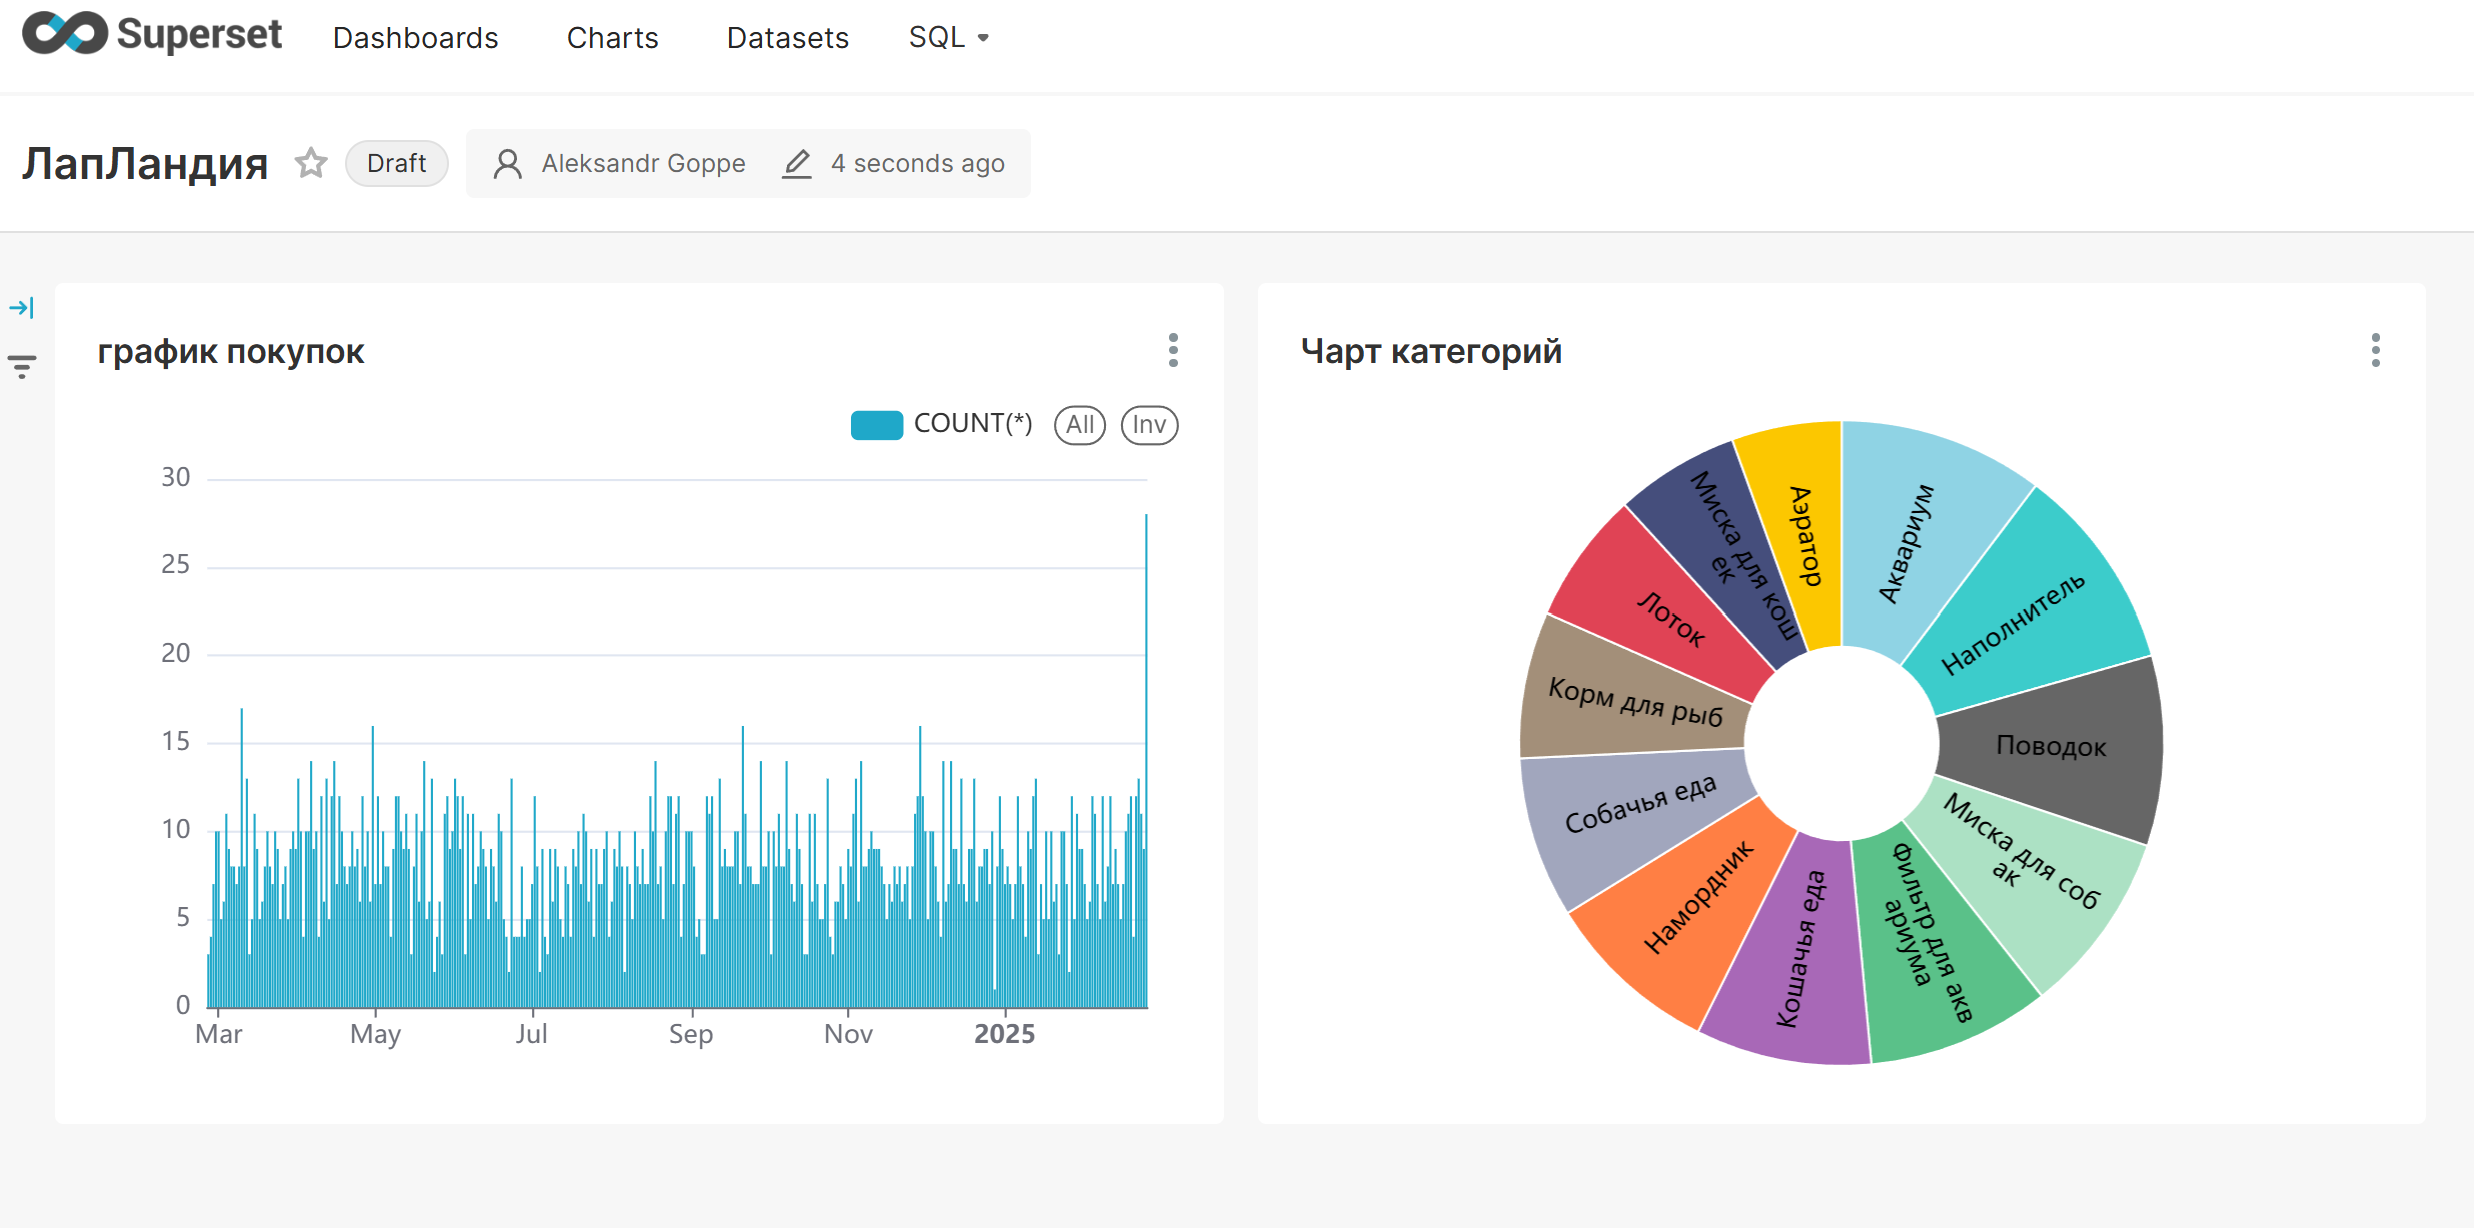
\includegraphics[width=0.9\textwidth]{superset} % Вставка изображения
    \caption{Панель в Superset}\label{fig:supersetpic}
\end{figure}

    \section{Демонстрационное серверное Java-приложение}\label{sec:-javaapp-}
    В демонстрационных целях было разработано веб-приложение, работающее с базами данных через актуальный подход
Spring-Boot+JPA и Hibernate.

\subsection{API приложения}\label{subsec:api-server-app}
В рамках демонстрационных задач в приложении объявлены эндпойнты по:
\begin{itemize}
    \item Получению базовой информации по продукту.
    \item Получению информации о покупках в рамках пагинации (через Slice).
    \item Получению информации о продуктах в рамках пагинации (через Page).
    \item Совершению случайной покупки - для презентации вставки данных в БД.
\end{itemize}

\subsection{Пагинация в контексте работы с БД}\label{subsec:jpapagination}

\subsubsection{Пагинация по умолчанию}\label{subsec:defaultpagination}
В базовой пагинации, реализованной в Spring Boot Jpa, как и во многих других,
в частности, Django в Python - используется извлечение через offset с запросом общего числа данных в таблице.
Это иллюстрируют записи в логе приложения от Hibernate, при выполнении запроса по продуктам:

\begin{lstlisting}[language=bash, frame=single, basicstyle=\normalsize\ttfamily, breaklines=true,label={lst:hiberpagelog}]
2025-03-02 13:23:22 Hibernate: select p1_0.id,p1_0.category_id,p1_0.characteristics,p1_0.description,p1_0.name,p1_0.price from business.product p1_0 offset ? rows fetch first ? rows only
2025-03-02 13:23:22 Hibernate: select count(p1_0.id) from business.product p1_0
\end{lstlisting}

На что можно обратить внимание:
\begin{itemize}
    \item При больших таблицах \textbf{offset} будет влиять на утилизацию ресурсов, т.к. БД будет арифметически
    идти по таблице, пока не придёт указателем на нужное место.
    \item Имеем дополнительный запрос на число записей, который не во всех сценариях ``прокрутки`` нужен клиенту.
\end{itemize}

\subsubsection{Использование keyset и slice}\label{subsec:slicekeysetpagination}
Можно использовать альтернативный запрос с использованием Slice вместо Page - тогда не будут производиться запросы
\textbf{count}, а также вместо offset использовать условие на какое-нибудь индексированное, удобное для упорядочивания
поле.
Например, числовой id.
В коде приложения это выглядит как код на HQL:
\begin{lstlisting}[language=java, frame=single, basicstyle=\normalsize\ttfamily, breaklines=true,label={lst:hqlquery}]
    @Query("""
            from Purchase p
              join fetch p.customer c
            where p.id > :lastId
            order by p.id asc
            limit :size
            """)
    Slice<Purchase> findByIdGreaterThanOrderByIdAsc(Integer lastId, int size);
\end{lstlisting}
Заметим, что благодаря использованию join fetch была устранена известная \textbf{N+1} проблема при использовании ORM,
когда при работе с связанными сущностями производятся дополнительные зопросы к БД для каждой сущности.

Теперь в логе видим:
\begin{lstlisting}[language=bash, frame=single, basicstyle=\normalsize\ttfamily, breaklines=true,label={lst:hiberpagelog}]
2025-03-02 14:48:54 Hibernate: select p1_0.id,p1_0.customer_id,c1_0.id,c1_0.bonus_points,c1_0.email,c1_0.loyalty_status,c1_0.name,c1_0.phone,p1_0.purchase_date,p1_0.shop_id,p1_0.total_amount from business.purchase p1_0 join business.customer c1_0 on c1_0.id=p1_0.customer_id where p1_0.id>? order by p1_0.id fetch first ? rows only
\end{lstlisting}

Без offset и count.

    \section{Сохранение логов в Clickhouse через Logstash}\label{sec:-logstashclickhouse-}
    \subsection{Общее описание механизма}\label{subsec:clickhousecommon}
В качестве дополнительного практического упражнения выполнено подключение выгрузки логов в Clickhouse через
Logstash.
Подобные подходы используются на практике, например в observability-платформе Sage.
Записи изначально поставляются в Logstash через logback-appender, настроенный в серверном приложении.
На нём же, в свою очередь, через кастомизацию docker-образа был установлен плагин для интеграции с Clickhouse.

\begin{figure}[htbp]
    \centering
    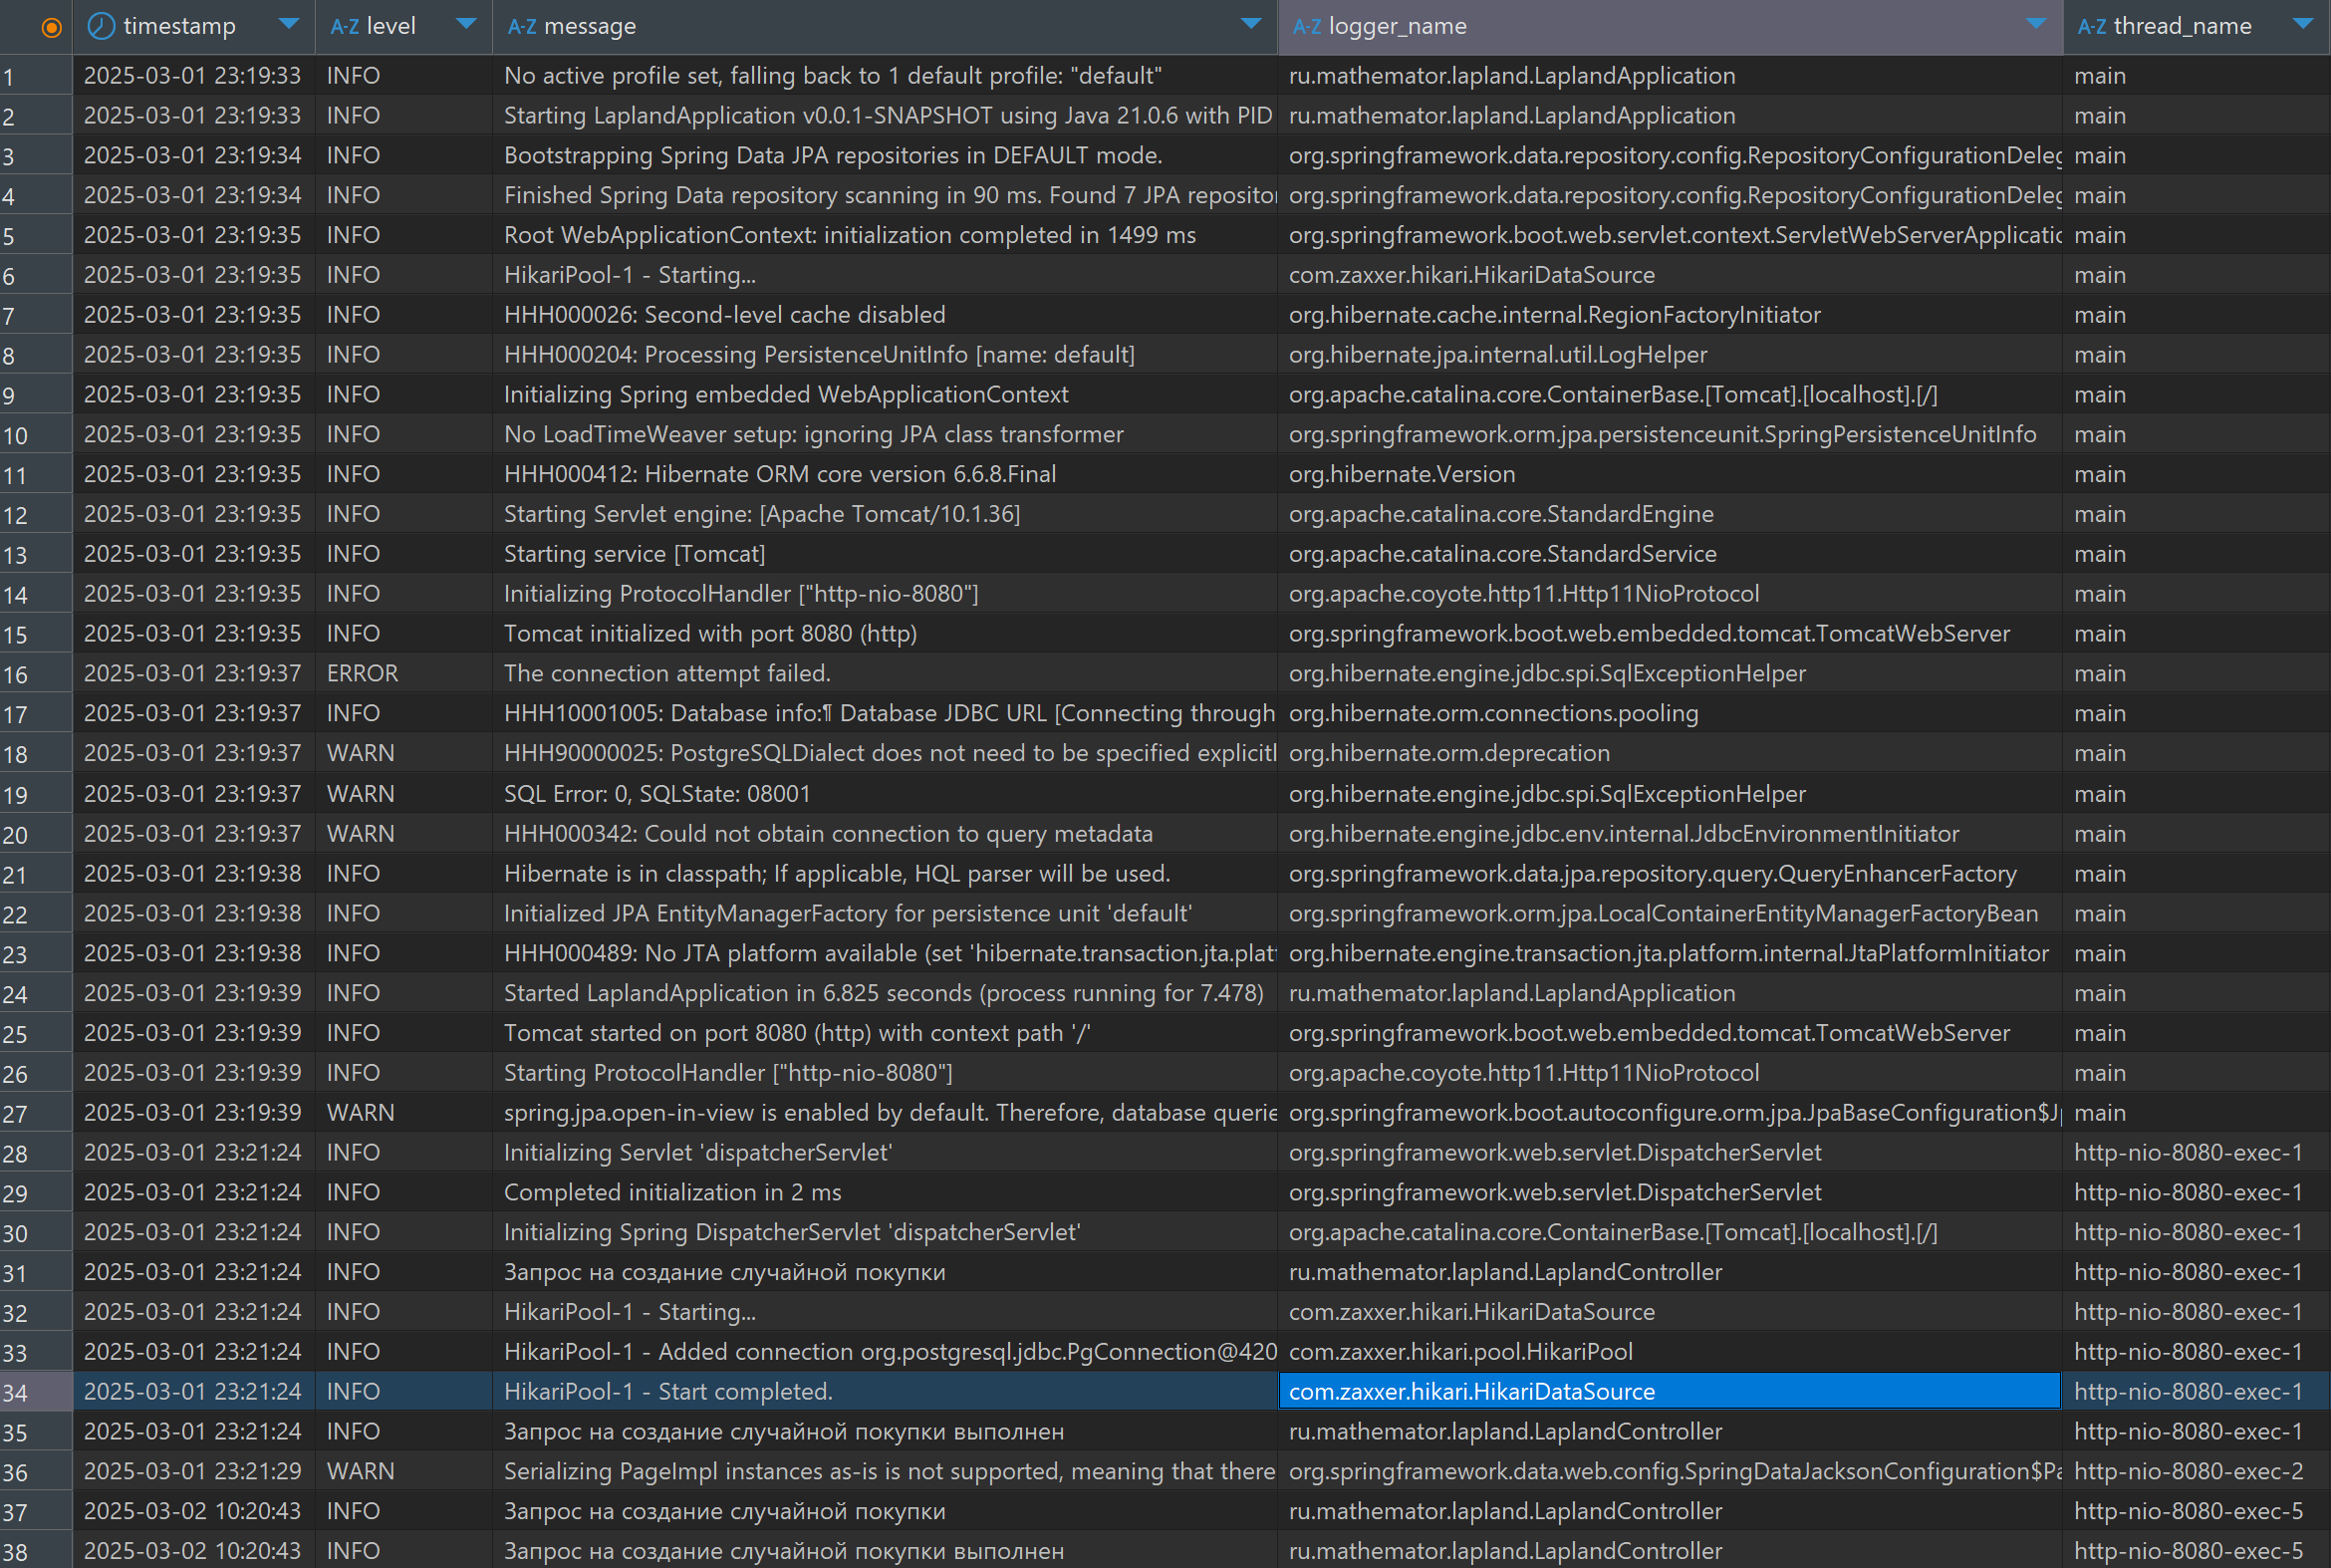
\includegraphics[width=0.9\textwidth]{clickhouse} % Вставка изображения
    \caption{Интерфейс DBeaver. Привычные логи Spring Boot приложения в таблице Clickhouse}\label{fig:clickhouse}
\end{figure}

\subsection{Нюансы настройки}\label{subsec:clickhousedetails}
В ходе развертывания решения возникла проблема в несоответствии timestamp-форматов, попадающих в Logstash и у
Clickhouse.
Для решения данной проблемы в конфигурацию был добавлен фильтр с функцией на ruby:
\begin{lstlisting}[language=ruby, frame=single, basicstyle=\normalsize\ttfamily, breaklines=true,label={lst:rubylist}]
event.set('timestamp', event.get('timestamp').time.localtime.strftime('%Y-%m-%d %H:%M:%S'))
\end{lstlisting}




    \section{Демонстрационное клиентское React.js-приложение}\label{sec:-reactapp-}
    \subsection{Общая информация о приложении}\label{subsec:frontcommon}
В качестве дополнительного, разивающего упражнения, с помощью инструментария Vite
разработано демонстрационное react.js-приложение, которое элегантно замыкает
разработку до ``человечного`` замкнутого решения.
В приложении доступны:
\begin{itemize}
    \item Кнопка совершения случайной покупки для демонстрации вставки в БД.
    \item Вкладка пагинированной таблицей товаров, нажатие на строки которой открывает страницу с описанием товара.
    \item Вкладка с пагинированной таблицей истории покупок.
\end{itemize}

Как отмечалось ранее, представления служат демонстрационным целям.
Также в приложении присутствует небольшое оформление, отражающее некоторые базовые правила UI/UX
касательно баланса цветов, рабочей зоны и привычных элементов интерфейса.

\begin{figure}[htbp]
    \centering
    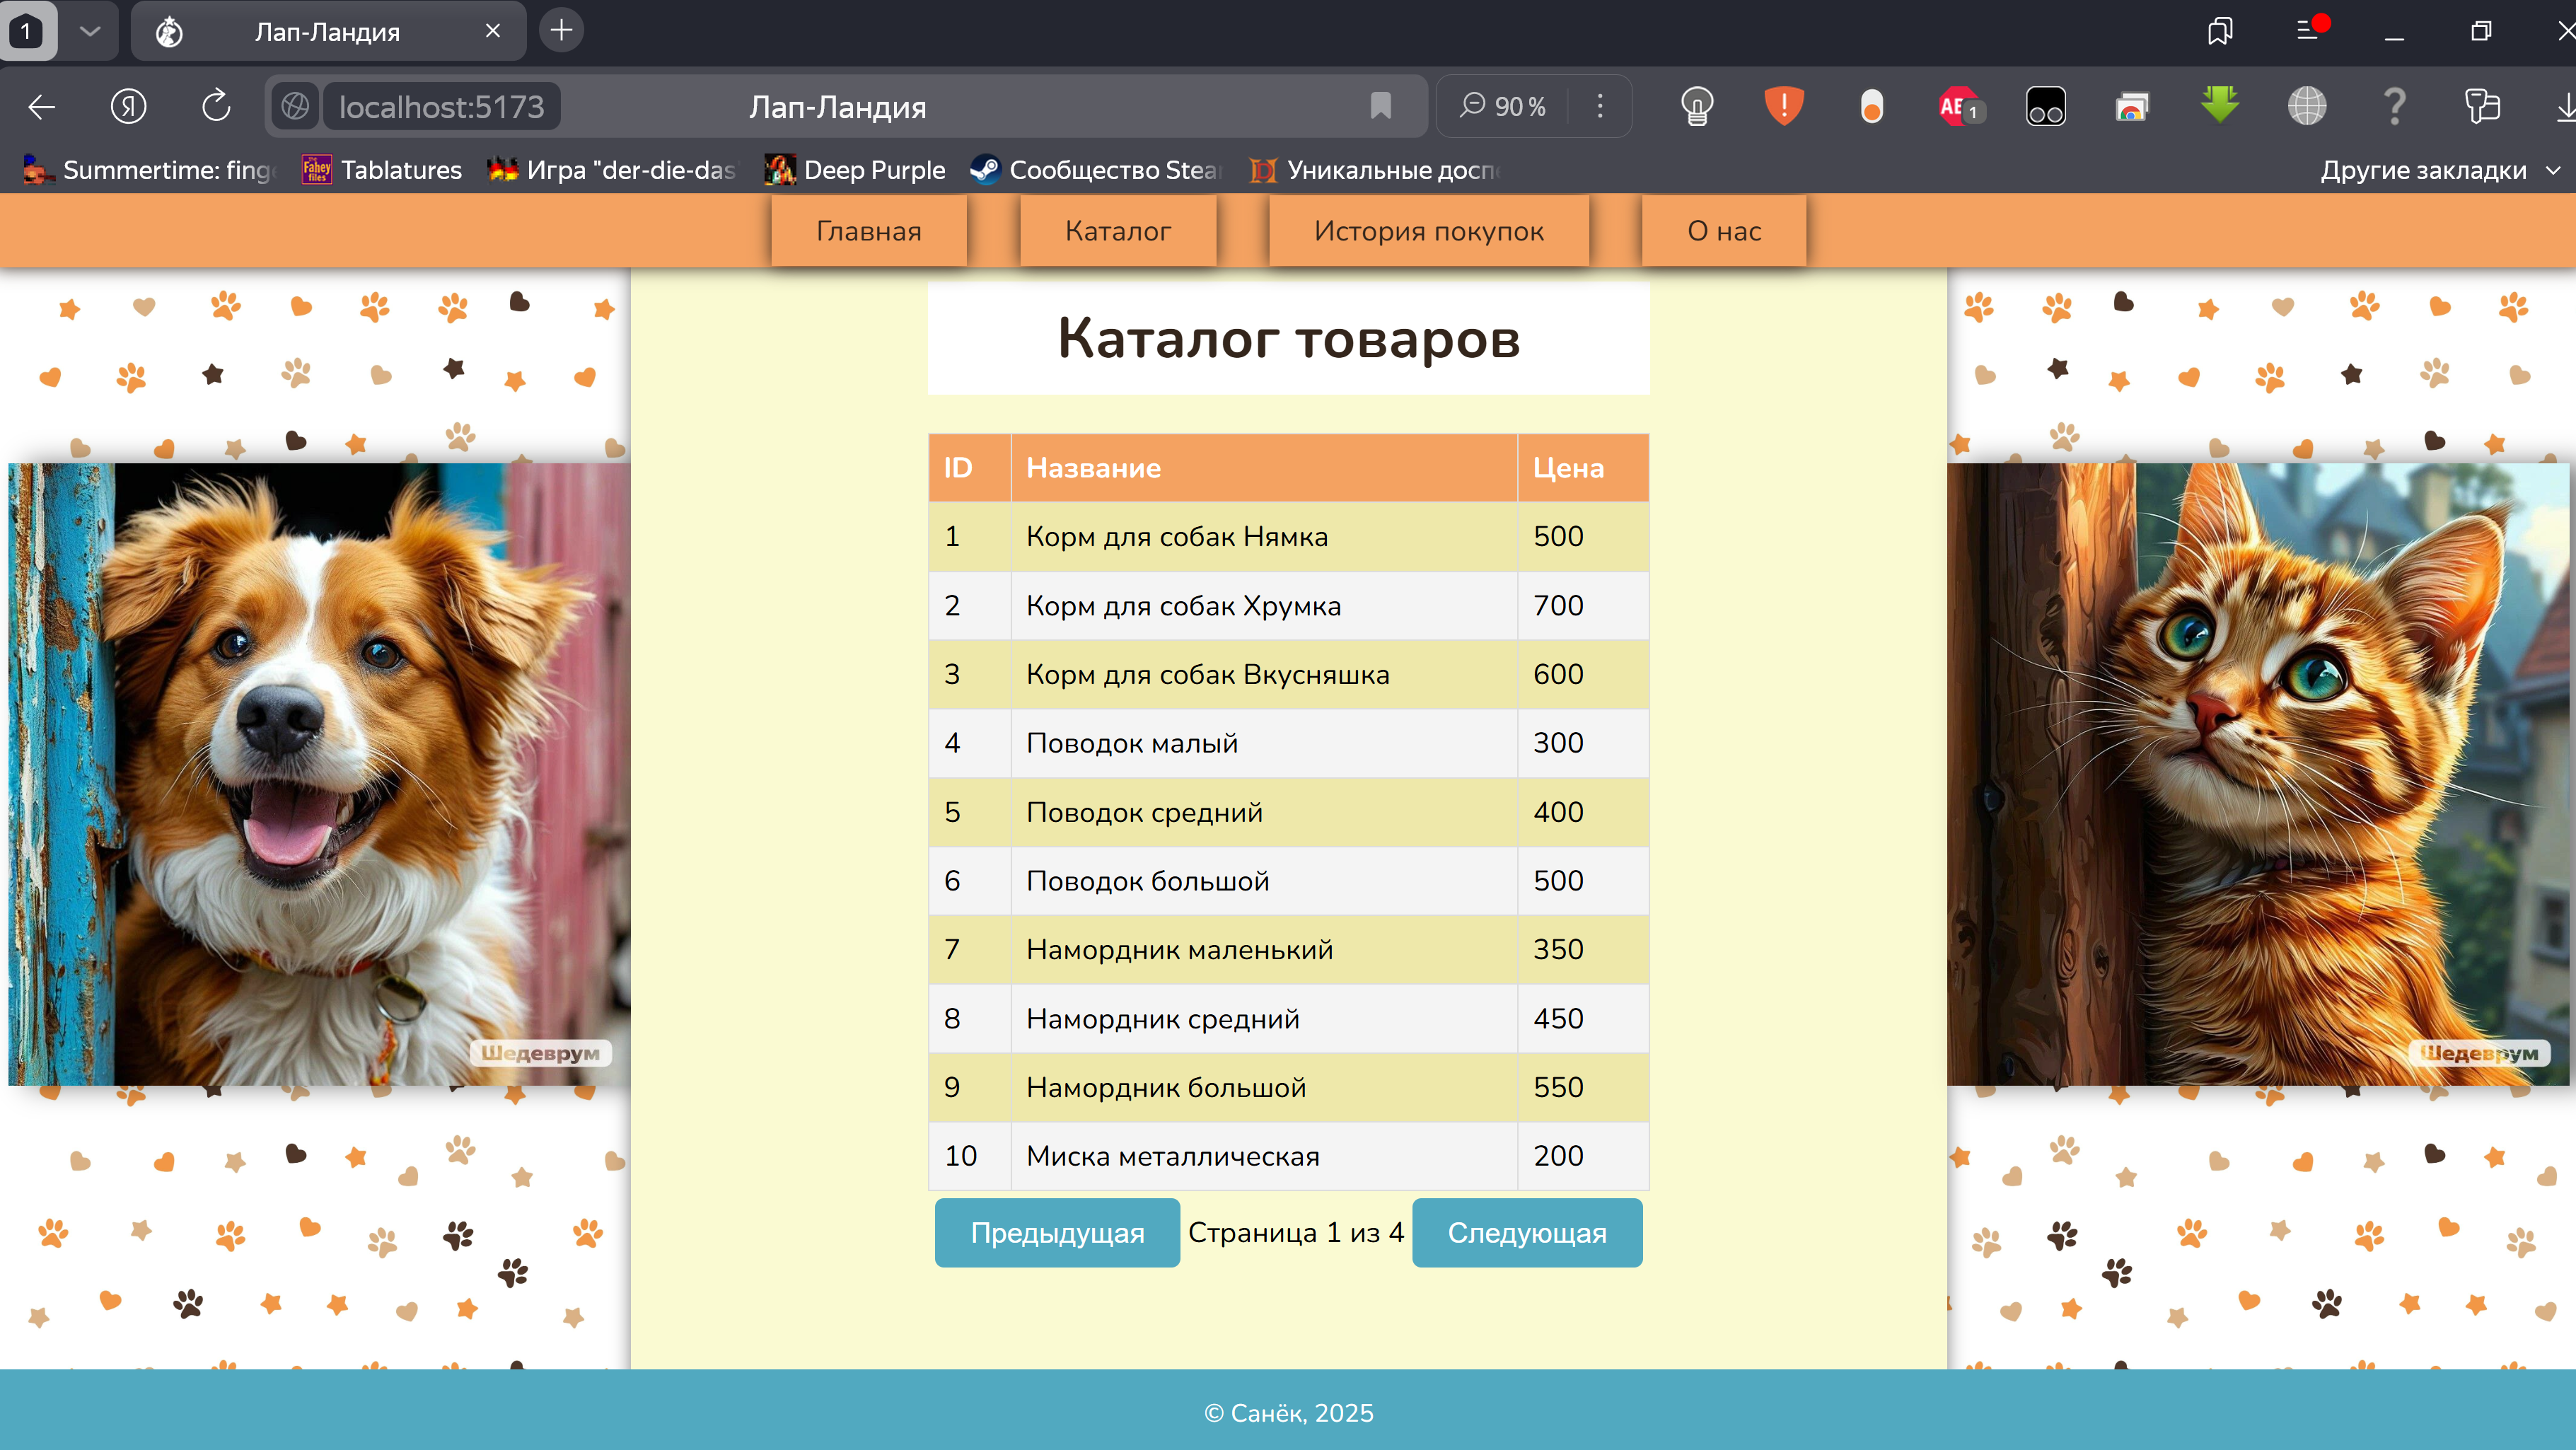
\includegraphics[width=0.9\textwidth]{browser} % Вставка изображения
    \caption{Снимок страницы клиентского приложения}\label{fig:browsershot}
\end{figure}

Изображения сгенерированы с помощью нейросети.
Иконка взята из открытых источников, со свободной лицензией.


    \section{Итоги}\label{sec:results}
    Вокруг целевой БД была настроена обширная инфраструктура, демонстрирующая как различные нюансы и аспекты, так
и, в целом, актуальные подходы при работе с базами данных.
Широкий спектр затрагиваемых вопросов наглядно подчёркивает необходимость развивать и поддерживать
компетенции в области БД для построения современных решений, основанных на работе с хранящимися цифровыми данными.

Спасибо за внимание!

\end{document}
